\documentclass{TDP005mall}
\usepackage{pdfpages}



\newcommand{\version}{Version 1.1}
\author{Josefin Bodin\\
  Alicia Bergman\\
Ahmed Sikh}
\title{Designspecifikation}
\date{\today}
\rhead{Josefin Bodin\\
  Alicia Bergman\\
Ahmed Sikh}


\begin{document}
\projectpage
\section{Revisionshistorik}
\begin{table}[!h]
\begin{tabularx}{\linewidth}{|l|X|l|}
\hline
Ver. & Revisionsbeskrivning & Datum \\\hline
1.1 & Färdig designspecifikation & 201217 \\\hline
1.0 & Första utkast & 201124 \\\hline
\end{tabularx}
\end{table}


\section{Detaljbeskrivning player}

Syftet med Player-klassen är att representera den karaktär som användaren
kontrollerar på spelplanen.  Den har utseendet av ett “kakmonster” och  styrs
genom den utritade labyrinten.

Player-klassen ärver funktionalitet från entity-klassen som i sin tur ärver från
objekt-klassen.


Konstruktorn som finns i Player tar inte in några parametrar. När ett objekt av
typen player skapas sätts texturen för spriten till den bild som ser ut som
karaktären. Förutom texturen sätts även skalan på spriten,
den har även en default position som spelaren får.
Förutom det får variablerna som representerar liv ett värde av 3 och hastigheten
får värdet 150.
I konstruktorn anropas även Entitys konstruktor, till den skickas bilden, skalan och positionen. 

De medlemsvariabler som player har är heltal variablerna points och lives.
Sedan har den också en float som heter speed, den har spelarens hastighet
lagrad.
Den innehåller även bool variabler som säger om spelaren kan flytta i en viss
riktning(canMoveUp, canMoveDown, canMoveRight och canMoveLeft).


Metoder som finns i klassen är bland annat input som sätter medlemsvariabler
till rätt värden beroende på den inmatning som användaren har gjort. I
Game-klassen skickas olika riktningar med beroende på vad användaren har matat
in.Input kallar på och kör move-funktionen.

I move så sker själva förflyttningen av spriten. Det kollas även så att spelaren
kan flytta på sig. Det finns även funktionerna get\_lives, set\_lives,
get\_points och set\_points för att de andra objekten skall kunna uppdateras vid
kollision. set\_speed är också en funktion som tillåter ändringa av spelarens
hastighet. Det finns även en metod som säger hur spelaren ska agera i de tillfällen
när den kolliderar med en vägg, den heter collision\_with\_wall. Update gör
ingenting i player.




\subsection{Entity}

Det som player ärver från entity är följande:

\begin{itemize}
  \item int move\_direction - En variabel som har värdet av den riktningen som
    spelaren rör sig i. De olika riktningar har fått nummer som representerar
    dem.
    
  \item sf::Time movement - En variabel till för att spelaren skall ha samma
    hastighet på olika datorer.
    
  \item virtual void move(sf::Time) = 0 - Funktion som inte har någon
    implementation i entity-klassen.
    
  \item virtual void update(sf::Time) = 0 - Funktion som inte har någon
    implementation i entity-klassen.
    
\end{itemize}

\subsection{Object}
Det som player ärver från objekt är följande:

\begin{itemize}
  \item  sf::Sprite sprite - Variabel som får en textur som representerar vår spelare.

  \item sf::Texture texture - Variable som håller våran texture.
    
  \item void draw(sf::RenderWindow\&) - Funktion som gör det möjligt att rita ut
    objekten.

  \item virtual void update(Player\&, sf::Time) = 0 - Funktion för att uppdatera spelaren.
    
  \item bool collision(Object const\&) const  - För att kolla om två objekt har
    kolliderat.

  \item sf::Sprite getsprite() const - Ger tillgång till spriten för alla objekt.
    
\end{itemize}


\section{Game}

I denna klassen körs hela spelet, den uppdaterar spelplanen och spelaren samt
tar hand om användarens inmatning. 

Game-kassen samarbetar mycket med world-klassen då det är den som håller all
objekten.

Det skickas in en parameter i konstruktorn som är namnet på den banan som ska
köras. Med den initieras ett world objekt som ligger i game. I klassens
konstruktor sätts även texten som kommer synas på skärmen som visar hur mycket
poäng och liv spelaren har i början av spelet. Den texten uppdateras under
spelets gång.

De medlems variabler som Game har är en bool som säger om spelet ska fortsätta
köras eller om det ska stängas ner. Det finns även variablerna sf::Text och
sf::Font har hand om hur texten som visas på skärmen ser ut och  en
sf::Clock och sf::Time som användes för att spelet ska köras likadant på alla
datorer. Det finns även ett objekt av typen world som håller alla objekten som
game ritar ut och uppdaterar.


Bland de metoder som Game har finns bland annat en funktion som heter run. Den
kör hela spelet. I run startas klockan för spelet om och de funktioner som
ligger i game kallas på. Input är en av dem, den tar den informationen som
ges när användaren trycker på knappar på tangentbordet. Beroende på inputen som
ges så skickas olika parametrar in till player för att den sedan ska röra sig. I
update-funktion så uppdateras spelet och uppdateringen ser annorlunda ut
beroende på om någon kollision sker. Det finns även en draw funktion som ritar
ut alla objekten som finns på spelplanen och funktioner som kollar
om spelaren har vunnit eller om det är game over. Detta kontrolleras i update-funktionen.


\section{Extern filhantering}

För att läsa in olika banor så skrivs de i en fil som läses in av
world-klassen. Den informationen som läses in från filen initierar nya objekt
som läggs på heapen och i vektorn finns pekare till de objekten.

\begin{center}
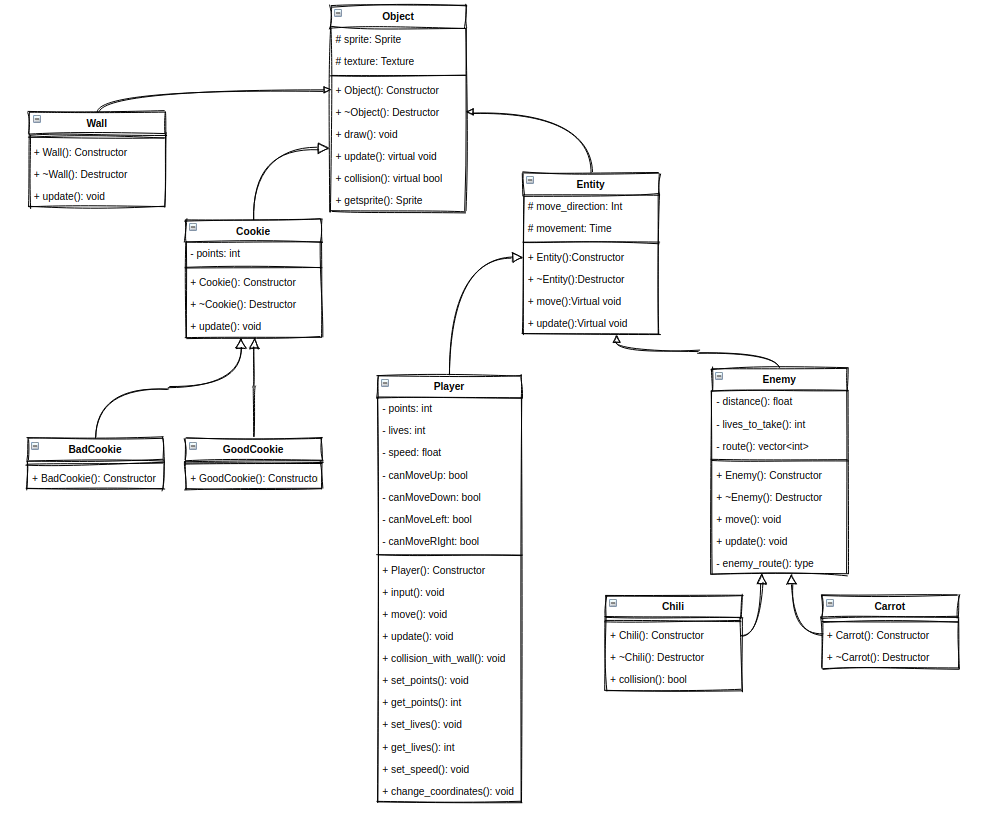
\includegraphics[scale=0.45]{umlObj.png}
\end{center}
\newpage
\begin{center}
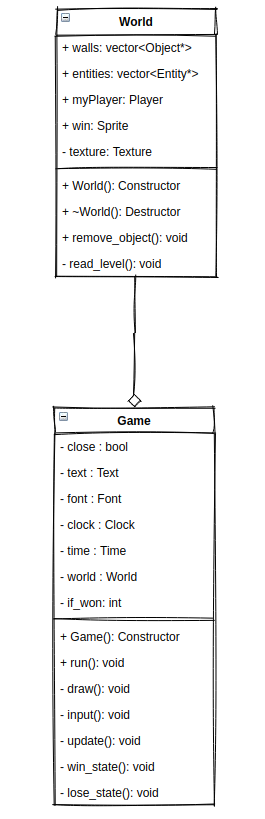
\includegraphics[scale = 0.5]{umlState.png}
\end{center}
\newpage
\begin{center}
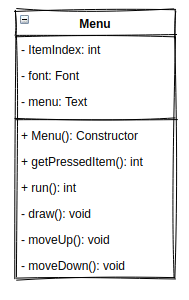
\includegraphics{umlMenu.png}
\end{center}
\newpage
\begin{center}
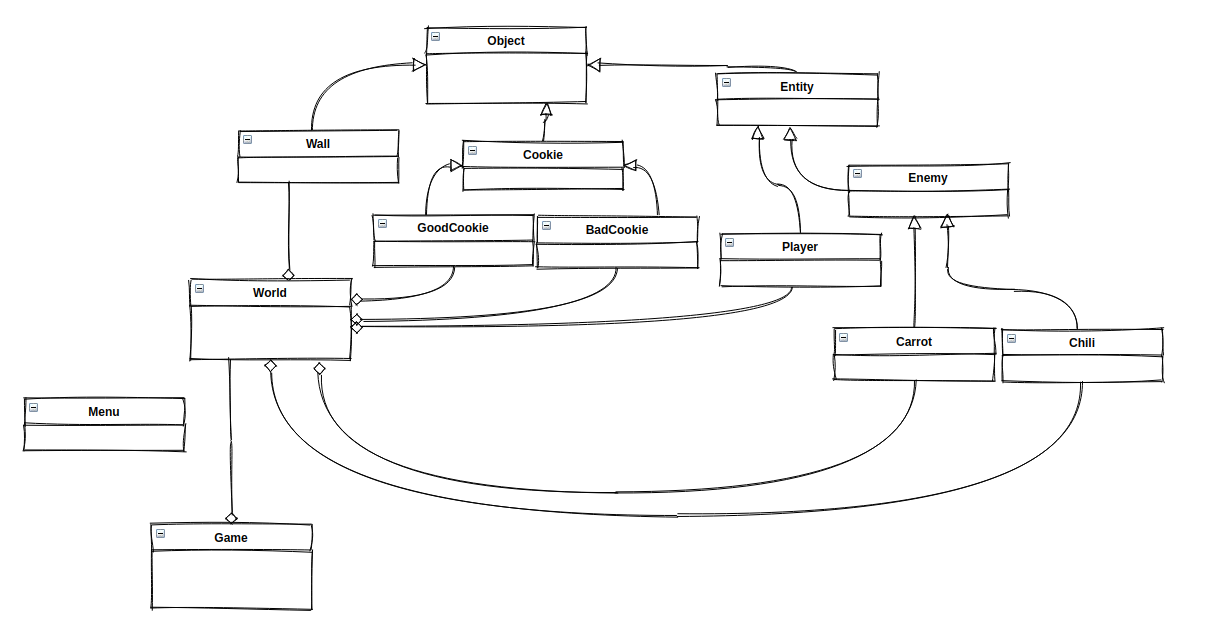
\includegraphics[scale = 0.45]{umlConnection.png}
\end{center}
\end{document}
